\begin{task}[credit=16]{Entscheidungsbäume - ID3 Algorithmus}
%\exercise{Entscheidungsbäume - ID3 Algorithmus}
%The table below shows making decision of playing baseball or not, based on four weather attributes.
Die folgende Tabelle zeigt die Entscheidung, ob Baseball gespielt wird, basierend auf vier Wetterattributen.

\begin{table}[h]
\centering
\caption{Trainingsdatensatz, ob Baseball gespielt wird basierend auf der Wetterlage.}
\label{tab:data_baseball}
\begin{tabular}{l|c|c|c|c|c}
\toprule
\textbf{Tag} & \textbf{Ausblick (A)} & \textbf{Temperatur (T)}  & \textbf{Luftfeuchtigkeit (L)} & \textbf{Wind (W)}     & \textbf{Spielt Baseball (B)} \\
\midrule
T1  & Sonnig    & Warm        & Hoch             & Schwach  & Nein            \\
T2  & Sonnig    & Warm        & Hoch             & Stark    & Nein            \\
T3  & Bewölkung & Warm        & Hoch             & Schwach  & Ja              \\
T4  & Regen     & Mild        & Hoch             & Schwach  & Ja              \\
T5  & Regen     & Kühl        & Normal           & Schwach  & Ja              \\
T6  & Regen     & Kühl        & Normal           & Stark    & Nein            \\
T7  & Bewölkung & Kühl        & Normal           & Stark    & Ja              \\
T8  & Sonnig    & Mild        & Hoch             & Schwach  & Nein            \\
T9  & Sonnig    & Kühl        & Normal           & Schwach  & Ja              \\
T10 & Regen     & Mild        & Normal           & Schwach  & Ja              \\
T11 & Sonnig    & Mild        & Normal           & Stark    & Ja              \\
T12 & Bewölkung & Mild        & Hoch             & Stark    & Ja              \\
T13 & Bewölkung & Warm        & Normal           & Schwach  & Ja              \\
T14 & Regen     & Mild        & Hoch             & Stark    & Nein            \\
\bottomrule
\end{tabular}
\end{table}

\begin{table}[h!]
\centering
\caption{Vorhersage-Datensatz, ob Baseball gespielt wird.}
\label{tab:data_baseball_predict}
\begin{tabular}{l|c|c|c|c|c}
\toprule
\textbf{Tag} & \textbf{Ausblick (A)} & \textbf{Temperatur (T)}  & \textbf{Luftfeuchtigkeit (L)} & \textbf{Wind (W)}     & \textbf{Spielt Baseball (B)} \\
\midrule
T15 & Sonnig    & Mild        & Hoch     & Schwach & ?       \\
T16 & Bewölkung & Mild        & Normal   & Schwach & ?       \\
T17 & Regen     & Kühl        & Normal   & Stark   & ?       \\
\bottomrule
\end{tabular}
\end{table}

%The target is to answer the question ``Should we play baseball?''
Die Aufgabe ist es folgende Frage zu beantworten: \textit{Unter welchen Bedingungen wir Baseball gespielt?}

%\begin{questions}
%\begin{question}{ID3 Algorithmus}{10}
\begin{subtask}[points=10,title=ID3 Algorithmus]
\label{q:id3_alg}
Erstellen Sie den Entscheidungsbaum mittels des ID3 Algorithmus.
Berechnen Sie dabei die \textbf{Entropie} und den \textbf{Informationsgewinn} (engl. \textit{gain}) der Attribut-Selektion für jeden Schritt.

\begin{solution}
Wir filtern im ersten Schritt nach Attributen und Schätzen $p_+$ und $p_-$ für jede Ausprägung des Attributs durch Zählen. Es ergibt sich
\begin{table}[H]
	\centering
	\caption{Attribut: Ausblick}
	\begin{tabular}{l|c|c|c|l}
		\toprule
		\textbf{Ausprägung} & \textbf{Anzahl} & \textbf{davon +}  & \textbf{davon -} &\textbf{Entropy} \\
		\midrule
		Sonnig    & 5 &2&3&0.971   \\
		Bewölkt & 4&4&0&0  \\
		Regen    & 5&3&2&0.971    \\
		\bottomrule
	\end{tabular}
\end{table}
\begin{table}[H]
	\centering
	\caption{Attribut: Temperatur}
	\begin{tabular}{l|c|c|c|c}
		\toprule
		\textbf{Ausprägung} & \textbf{Anzahl} & \textbf{davon +}  & \textbf{davon -} &\textbf{Entropy} \\
		\midrule
		Warm  & 4 &2&2&1      \\
		Mild & 6&4&2&0.918   \\
		Kühl & 4&3&1&0.811    \\
		\bottomrule
	\end{tabular}
\end{table}
\begin{table}[H]
	\centering
	\caption{Attribut: Luftfeuchtigkeit}
	\begin{tabular}{l|c|c|c|c}
		\toprule
		\textbf{Ausprägung} & \textbf{Anzahl} & \textbf{davon +}  & \textbf{davon -} &\textbf{Entropy} \\
		\midrule
		Hoch  & 7 &3&4&0.985      \\
		Normal & 7&6&1&0.591   \\
		\bottomrule
	\end{tabular}
\end{table}
\begin{table}[H]
	\centering
	\caption{Attribut: Wind}
	\begin{tabular}{l|c|c|c|c}
		\toprule
		\textbf{Ausprägung} & \textbf{Anzahl} & \textbf{davon +}  & \textbf{davon -} &\textbf{Entropy} \\
		\midrule
		Stark  & 6 &3&3&1      \\
		Schwach &8&6&2&0.811   \\
		\bottomrule
	\end{tabular}
\end{table}
Pro Ausprägung setzen wir nun
\begin{align*}
p_+=\frac{\text{davon +}}{\text{Anzahl}}\;\;\; \text{und}\;\;\; p_-=\frac{\text{davon -}}{\text{Anzahl}}
\end{align*}
und berechnen die Entropien mittels $I(p_+,p_-)=(-p_+\cdot\log p_+)+(-p_-\cdot\log p_-)$. Wobei der Logarithmus zur Basis 2 benutzt wurde. Die Ergebnisse haben wir an die Tabelle angefügt. Letztlich finden wir für jedes Attribut Att. den Informationsgehalt mittels \begin{align*}
\text{Information}(\text{Att.})=-\sum_{\text{Ausprägung A von Att.}}\frac{\text{Anzahl(A)}}{\text{ges}}\cdot\text{Entropy(A)}
\end{align*}
Es ergibt sich (ges=14),
\begin{table}[H]
	\centering
	\caption{Informationsgehalt}
	\begin{tabular}{l|c}
		\toprule
		\textbf{Attribut} & \textbf{Information}  \\
		\midrule
		Ausblick & -0.694\\
		Temperatur & -0.911\\
		Luftfeuchtigkeit & -0.788\\
		Wind&-0.892\\
		\bottomrule
	\end{tabular}
\end{table}
, sodass wir uns als erstes Kriterium für das Attribut Ausblick entscheiden. Bei Bewölkung sind bereits alle Tage in einer Kategorie (+), weshalb wir hier ein Blatt mit einem + erstellen. Betrachten wir nun also alle Tage an denen es Sonnig ist und erstellen hier rekursiv einen Teilbaum. Wir fassen nochmal alle Daten, welche wir in diesem Knoten gegeben haben zusammen:
\begin{table}[H]
	\centering
	\caption{Trainingsdatensatz, nur Sonnig}
	\begin{tabular}{l|c|c|c|c|c}
		\toprule
		\textbf{Tag} & \textbf{Ausblick (A)} & \textbf{Temperatur (T)}  & \textbf{Luftfeuchtigkeit (L)} & \textbf{Wind (W)}     & \textbf{Spielt Baseball (B)} \\
		\midrule
		T1  & Sonnig    & Warm        & Hoch             & Schwach  & Nein            \\
		T2  & Sonnig    & Warm        & Hoch             & Stark    & Nein            \\
		T8  & Sonnig    & Mild        & Hoch             & Schwach  & Nein            \\
		T9  & Sonnig    & Kühl        & Normal           & Schwach  & Ja              \\
		T11 & Sonnig    & Mild        & Normal           & Stark    & Ja              \\
		\bottomrule
	\end{tabular}
\end{table}
Wir zählen, so wie oben und erhalten:
\begin{table}[H]
	\centering
	\caption{nur Sonnig, Attribut: Temperatur}
	\begin{tabular}{l|c|c|c|c}
		\toprule
		\textbf{Ausprägung} & \textbf{Anzahl} & \textbf{davon +}  & \textbf{davon -} &\textbf{Entropy} \\
		\midrule
		Warm  & 2 &0&2&0      \\
		Mild & 2&1&1&1   \\
		Kühl & 1&1&0&0    \\
		\bottomrule
	\end{tabular}
\end{table}
\begin{table}[H]
	\centering
	\caption{nur Sonnig, Attribut: Luftfeuchtigkeit}
	\begin{tabular}{l|c|c|c|c}
		\toprule
		\textbf{Ausprägung} & \textbf{Anzahl} & \textbf{davon +}  & \textbf{davon -} &\textbf{Entropy} \\
		\midrule
		Hoch&3&0&3&0\\
		Normal&2&2&0&0\\
		\bottomrule
	\end{tabular}
\end{table}
\begin{table}[H]
	\centering
	\caption{nur Sonnig, Attribut: Wind}
	\begin{tabular}{l|c|c|c|c}
		\toprule
		\textbf{Ausprägung} & \textbf{Anzahl} & \textbf{davon +}  & \textbf{davon -} &\textbf{Entropy} \\
		\midrule
		Schwach&3&1&2&0.918\\
		Stark&2&1&1&1\\
		\bottomrule
	\end{tabular}
\end{table}
Man sieht direkt, dass Attribut L auf den Trainingsdaten eine optimalen Informationsgewinn hat. Dies verifiziert man durch Berechnen der Informationsgehalte(ges=5)):
\begin{table}[H]
	\centering
	\caption{Informationsgehalt, nur Sonnig}
	\begin{tabular}{l|c}
		\toprule
		\textbf{Attribut} & \textbf{Information}  \\
		\midrule
		Temperatur&-0.4\\
		Luftfeuchtigkeit & 0\\
		Wind&-0.95\\
		\bottomrule
	\end{tabular}
\end{table}
Unter dem Sonnig-Ast erzeugen wir also einen Knoten 'Luftfeuchtigkeit' mit 2 Blättern. Ast 'hoch' führt zu - und Ast 'normal' zu +.\\
Nun müssen wir noch den Teilbaum finden, der an den Ast 'Regen' anhängt. Filtern wir also nach diesem Attribut und zählen dann wieder, so erhalten wir:
\begin{table}[H]
	\centering
	\caption{Trainingsdatensatz, nur Regen}
	\begin{tabular}{l|c|c|c|c|c}
		\toprule
		\textbf{Tag} & \textbf{Ausblick (A)} & \textbf{Temperatur (T)}  & \textbf{Luftfeuchtigkeit (L)} & \textbf{Wind (W)}     & \textbf{Spielt Baseball (B)} \\
		\midrule
		T4  & Regen     & Mild        & Hoch             & Schwach  & Ja              \\
		T5  & Regen     & Kühl        & Normal           & Schwach  & Ja              \\
		T6  & Regen     & Kühl        & Normal           & Stark    & Nein            \\
		T10 & Regen     & Mild        & Normal           & Schwach  & Ja              \\
		T14 & Regen     & Mild        & Hoch             & Stark    & Nein            \\
		\bottomrule
	\end{tabular}
\end{table}
\begin{table}[H]
	\centering
	\caption{nur Regen, Attribut: Temperatur}
	\begin{tabular}{l|c|c|c|c}
		\toprule
		\textbf{Ausprägung} & \textbf{Anzahl} & \textbf{davon +}  & \textbf{davon -} &\textbf{Entropy} \\
		\midrule
		Mild & 3&2&1&0.918   \\
		Kühl & 2&1&1&1    \\
		\bottomrule
	\end{tabular}
\end{table}
\begin{table}[H]
	\centering
	\caption{nur Regen, Attribut: Luftfeuchtigkeit}
	\begin{tabular}{l|c|c|c|c}
		\toprule
		\textbf{Ausprägung} & \textbf{Anzahl} & \textbf{davon +}  & \textbf{davon -} &\textbf{Entropy} \\
		\midrule
		Hoch&2&1&1&1\\
		Normal&3&2&1&0.918\\
		\bottomrule
	\end{tabular}
\end{table}
\begin{table}[H]
	\centering
	\caption{nur Regen, Attribut: Wind}
	\begin{tabular}{l|c|c|c|c}
		\toprule
		\textbf{Ausprägung} & \textbf{Anzahl} & \textbf{davon +}  & \textbf{davon -} &\textbf{Entropy} \\
		\midrule
		Schwach&3&3&0&0\\
		Stark&2&0&2&0\\
		\bottomrule
	\end{tabular}
\end{table}
Wir sehen wieder direkt die perfekte Klassifizierung beim Attribut Wind(Informationswert=0). Die anderen beiden haben jeweils einen Informationswert von -0.951. Wir erstellen hier also einen Knoten 'Wind' mit 2 Blättern '+' für Ausprägung 'schwach' und '-' für Ausprägung 'stark'.
\end{solution}

\end{subtask}

\begin{subtask}[points=3,title=Visualisierung]
Erstellen Sie eine Visualisierung (Plot oder eingefügte Zeichnung) des Entscheidungsbaumes aus Aufgabenteil~\ref{q:id3_alg}.

\begin{solution}
Es ergab sich insgesamt der folgende Entscheidungsbaum:
\begin{figure}[H]
	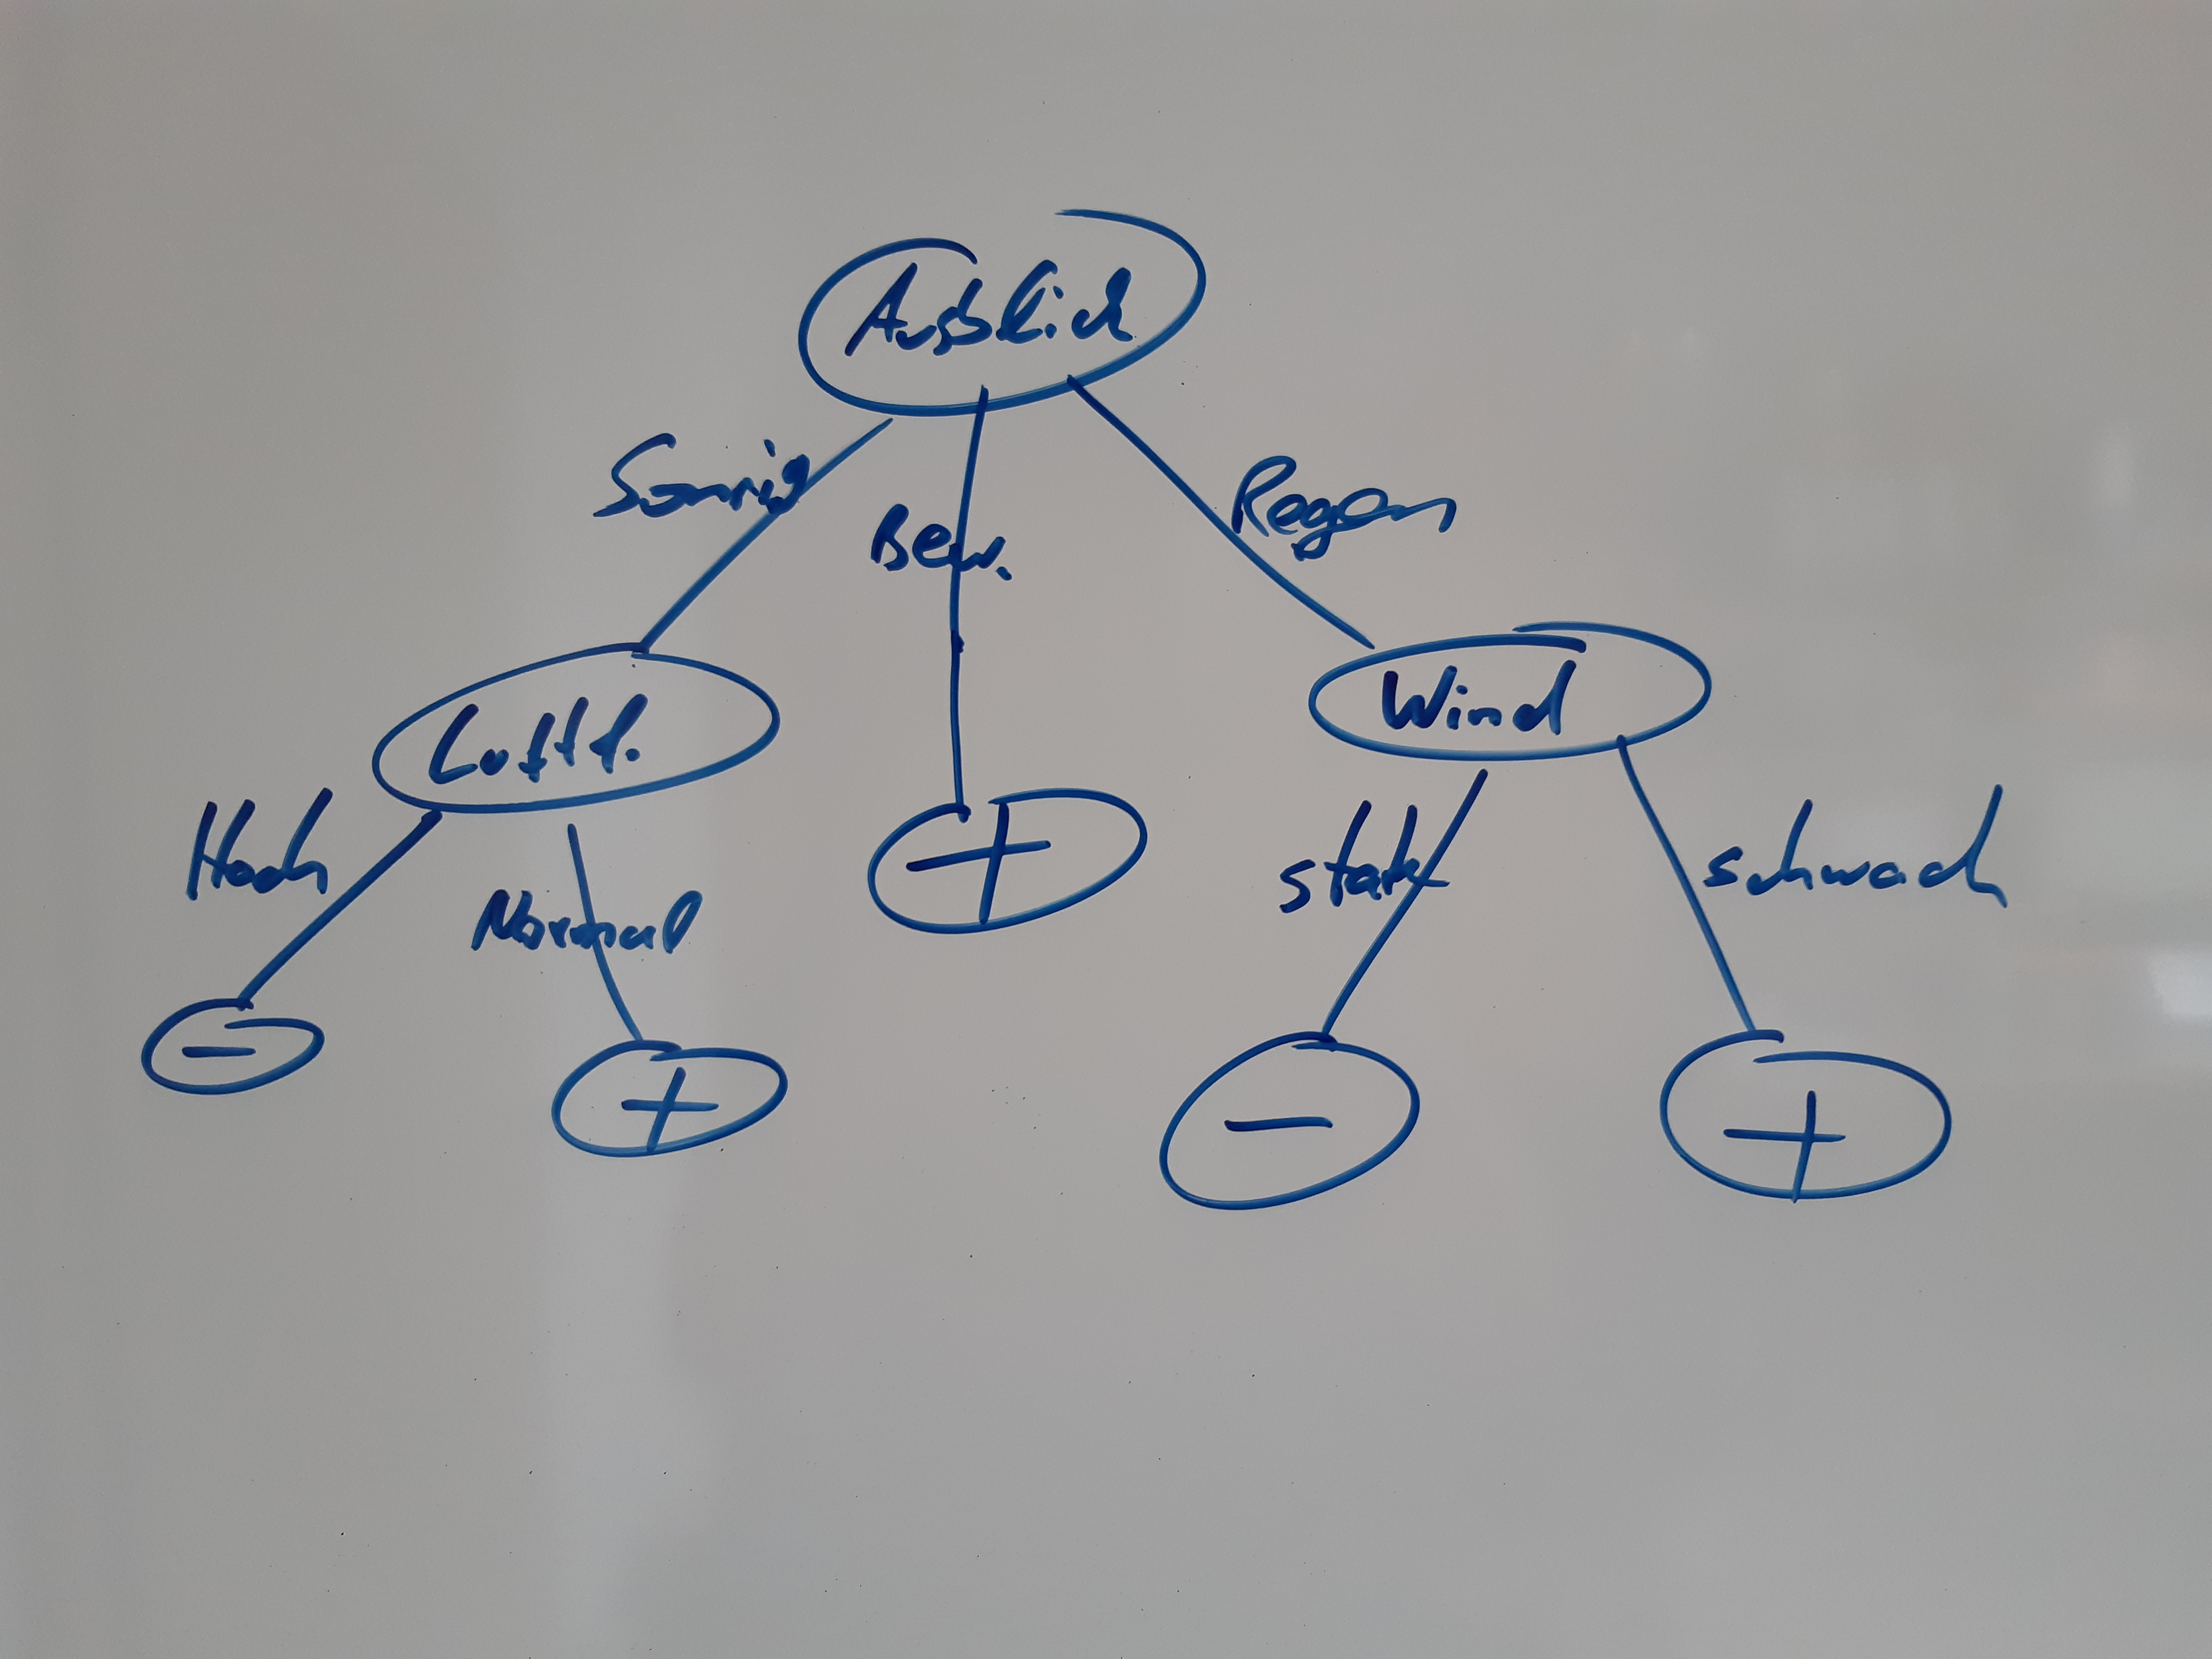
\includegraphics[width=0.5\textwidth]{1a.jpg}
\end{figure}
\end{solution}

\end{subtask}

\begin{subtask}[points=3,title=Vorhersage]
Geben Sie anhand ihres Entscheidungsbaumes eine Vorhersage für die Tage 15 bis 17 aus Tabelle~\ref{tab:data_baseball_predict}, ob Baseball gespielt wird.

\begin{solution}
% Geben sie hier ihre Antwort an.
\end{solution}

\end{subtask}
\end{task}